\chapter{Aufgabe 1}

\section{Teil a)}

\textit{Wie kann vertrauliche Kommunikation innerhalb einer Gruppe etabliert werden?}\\

\noindent
Bei \textbf{PGP} (\textit{Pretty Good Privacy}) werden Identitäten an einen Schlüssel gebunden: Diese Bindungen bestehen dann aus einem Datensatz, der mindestens

\begin{itemize}
    \itemsep0.5em
    \item einen öffentlichen Schlüssel
    \item eine Identität
    \item eine Signatur
\end{itemize}

\noindent
beinhaltet (vgl.~\cite[43]{ITS6}).\\

\noindent
Wir gehen in unserem Fall davon aus, dass die \textit{Identität} der Datensätze durch die Email-Adresse der Studenten gegeben ist.\\

\noindent
Zudem soll als \textit{vertrauenswürdige Instanz} jeder Student selber gelten: Diese erstellen Signatur und Zertifikate selber.\\
Da die Studenten zudem in (kleinere) Gruppen unterteilt worden sind, können die Studenten innerhalb der Gruppe ihr gegenseitiges Vertrauen durch gegenseitiges signieren der selbst erstellten Zertifikate ausdrücken - an dieser Stelle sei angemerkt, dass es sich hierbei eher um einen Formalismus handelt, d.h. es wird in erster Linie keine \textit{freundschaftliche} Vertrauensbasis aufgebaut, sondern das Vertrauen wird durch gegenseitige, persönliche Überprüfung der Identität - bspw. anahnd von den Dokumenten Personal- und Studenentenausweis beim Treffen von Übungsgruppen - hergestellt.
Das ganze ist in Abbildung~\ref{fig:weboftrust} schematisch dargestellt: In der Gruppe $1$ existieren $5$ Studenten, die ihr Zertifikat selbst signiert haben, ausgedrückt durch eine reflexive Kante. \\
Bei einem persönlichen Treffen wird die Identität der Teilnehmer gegenseitig überprüft und danach das \textbf{Web-of-Trust} durch gegenseitiges signieren der Zertifikate erstellt - Student $E_1$ stößt später zu der Gruppe hinzu und vertraut Student $A_1$ (gegenseitiges Signieren der Zertifikate).
Durch $A_1$ wird damit  implizit das Vertrauen zu den übrigen Studenten hergestellt wird (gestrichelte Linie in der Abbildung).\\

\noindent
Insgesamt kann durch dieses Verfahren vertrauliche Kommunikation hergestellt werden: Öffentliche Schlüssel der Teilnehmer einer Gruppe sind als \textit{vertrauenswürdig} eingestuft und durch die Bindung and die Identität wird die \textit{Authentizität} der Schlüssel sichergestellt.
Bei der Kommunikation werden individuelle private Schlüssel zur Signatur der Nachrichten verwendet, die mittels der (zertifizierten) öffentlichen Schlüssel überprüft werden können.\\
Gleichzeitig werden die Nachrichten mit den öffentlichen Schlüsseln der jeweiligen Empfänger verschlüsselt: Auch hier ist durch die Zertifikate die \textit{Authentizität} sichergestellt.

\begin{figure}
    \centering
    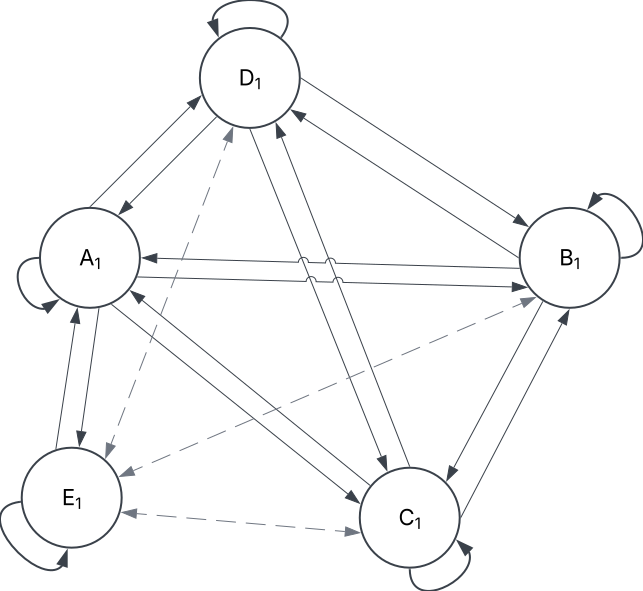
\includegraphics[scale=0.4]{aufgabe 1/img/weboftrust.svg}
    \caption{Studenten signieren in dem gegebenen Szenario die PGP-Zertifikate gegenseitig. (Quelle: eigene)}
    \label{fig:weboftrust}
\end{figure}

\noindent
Um die vertrauliche Kommunikation \textbf{innerhalb} der Gruppe zu garantieren, so dass auch mehrere Empfänger  andere Gruppen der Hochschule, die nach dem gleichen Prinzip ihre \textit{Web-of-Trusts} aufbauen, kann (mit dem o.a. Beispiel) wie folgt vorgegangen werden - hierbei ist $X_n$ ein Außenstehender, der nicht innerhalb des Web-of-Trust der Gruppe $1$ existiert, und für den die Kommunikation zwischen $A_1$ und $B_1$ aufgrund der Vertraulichkeit von Gruppe $1$ verborgen bleiben soll.

\begin{enumerate}
    \itemsep0.5em
    \item $A_1$ erstellt eine Nachricht $m$ an $B_1$ und $C_1$.
    \item $A_1$ erstellt einen einmaligen, randomisierten Sitzungsschlüssel $K_s$.
    \item $K_s$ wird genutzt, um $m$ zu $E_{K_s}(m)$verschlüsseln.
    \item Für jedes Gruppenmitglied $G_i$, an das die Nachricht geht, wird $K_s$ mit dem öffentlichen Schlüssel $OS_i$ der Empfänger verschlüsselt: Es entstehen
    \begin{itemize}
        \item die asymmetrisch verschlüsselten Sitzungsschlüssel $E_{OS_i}(K_s)$
        \item die durch $\text{PrivS}_{A_1}$ signierte verschlüsselte Nachricht $\text{Sig}_{A_1}(E_{K_s}(m))$
    \end{itemize}
    \item $G_i$ erhalten die Nachrichten $\text{Sig}_{A_1}(E_{K_s}(m))||E_{OS_i}(K_s)$, darunter $B_1$: Die Signatur der Nachricht wird mittels $OS_{A_1}$ überprüft.
    \item Der asymmetrisch verschlüsselte \textit{symmetrische} Schlüssel wird mit $\text{PrivS}_{B_1}$ entschlüsselt.
    \item Die Nachricht wird entschlüsselt und gelesen.
\end{enumerate}

\section{Teil b)}

\textit{Wie ist vorzugehen, wenn Mitglieder aus der Gruppe ausscheiden?}\\

\noindent
Wenn Mitglieder aus der Gruppe ausscheiden muss sichergestellt werden, dass dies den Gruppenteilnehmern kommuniziert werden: Hierdurch sollen die ``Verbindungen`` zu den Knoten aufgelöst werden, die fortan nicht mehr in der Gruppe existieren und deshalb als nicht mehr vertrauenswürdig eingestuft werden können.
Hierbei können \textit{CRL} (\textit{Certificate Revocation Lists},~\cite[34 f.]{ITS6}) helfen, die Zertifikate als ungültig markieren.
Eine Einbindung und ein regelmäßiger Abgleich dieser Widerrufslisten kann zur Automatisierung des Prozesses und zur Pflege der SIS beitragen.\\
Dies ist insbesondere im Hinblick auf das \textit{Web-of-Trust} von Bedeutung: Scheidet der in Abbildung~\ref{fig:weboftrust} dargestellte Teilnehmer $C_1$ aus und erfährt die Verbindung zwischen $A_1$ und $C_1$ keinen Zertifikatswiderrruf, so würde $E_1$ weiterhin $C_1$ (notwendigerweise) als vertrauenswürdig einordnen, da er diese Einstufung ausschließlich über $A_1$ erhält.